% Created 2021-01-24 Sun 22:49
% Intended LaTeX compiler: pdflatex
\documentclass[11pt]{article}
\usepackage[utf8]{inputenc}
\usepackage[T1]{fontenc}
\usepackage{graphicx}
\usepackage{grffile}
\usepackage{longtable}
\usepackage{wrapfig}
\usepackage{rotating}
\usepackage[normalem]{ulem}
\usepackage{amsmath}
\usepackage{textcomp}
\usepackage{amssymb}
\usepackage{capt-of}
\usepackage{hyperref}
\usepackage{minted}
\hypersetup{colorlinks=true, linkcolor=black, filecolor=red, urlcolor=blue}
\usepackage[turkish]{babel}
\author{Eren Hatırnaz}
\date{15 Haziran 2020}
\title{Yazılım Gündemi - 2020/23\\\medskip
\large 8-14 Haziran 2020}
\hypersetup{
 pdfauthor={Eren Hatırnaz},
 pdftitle={Yazılım Gündemi - 2020/23},
 pdfkeywords={},
 pdfsubject={},
 pdfcreator={Emacs 27.1 (Org mode 9.3)},
 pdflang={Turkish}}
\begin{document}

\maketitle
\tableofcontents \clearpage\shorthandoff{=}

\begin{center}
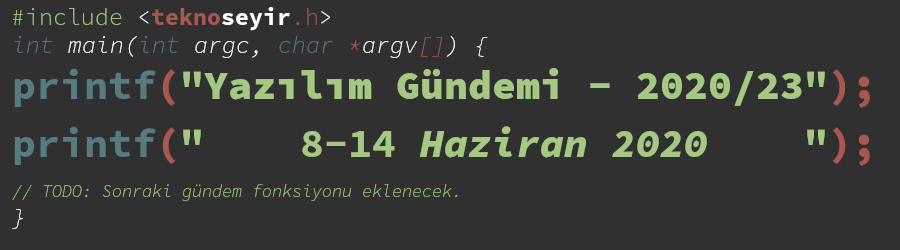
\includegraphics[width=.9\linewidth]{gorseller/yazilim-gundemi-banner.png}
\end{center}

\begin{center}
\href{../22/yazilim-gundemi-2020-22.pdf}{< Önceki Gündem} | \textbf{8-14 Haziran 2020} | \href{../24/yazilim-gundemi-2020-24.pdf}{Sonraki Gündem >}

\href{https://teknoseyir.com/blog/yazilim-gundemi-2020-23}{TeknoSeyir'de Oku}
\end{center}

\section{PHP \href{https://www.jetbrains.com/lp/php-25/}{25 yaşında} ve PHP 8 sürümü \href{https://externals.io/message/110470}{yayın takvimi yayınlandı}}
\label{sec:orgbf441ae}
Geçtiğimiz hafta içerisinde PHP programlama dili 25 yaşına girdi. Yani
yaratıcısı Rasmus Lerdorf'un Personal Home Page Tools adı altında kendi
kişisel ihtiyaçları için geliştirdiği C kütüphanesinin ilk sürümünün
yayınlanmasının ardından 25 yıl geçti. Bugün ise web arka yüz (back-end)
tarafında en çok kullanılan programlama dillerinden birisi haline gelmiş
durumda. JetBrains firması da PHP'nin \href{https://www.jetbrains.com/lp/php-25/}{25 yıllık hikayesini anlatan bir sayfa}
hazırladı. Mutlaka göz atmanızı tavsiye ederim. Ben de PHP ile yaşıtım :)

Ben de programlamaya derinlemesine merak salmadan önce ortaokuldayken forum
siteleri açıp, kapatmakla uğraşıyordum sürekli. phpBB, MyBB, SMF (Simple
Machines Forum) ve vBullettin gibi birçok forum altyapıysa uğraştım. Bunları
özelleştirdim, eklentiler geliştirdim fakat maalesef açtığım hiçbir forum
sitesi tutmadı. Hepsi PHP ile geliştirilmiş sistemler olduğu için tabii bir
miktar PHP de öğrenmiş oldum. Sonraları programlamaya ilgim daha da arttı ama
o zamanlarda güzel zamanlardı :). Paket yönetim sistemleri ve standardizasyon
çalışmalarından önceki PHP gerçekten zor zamanlar yaşatıyordu insanlara ama
\href{https://getcomposer.org/}{Composer} ve \href{https://www.php-fig.org/}{PHP-FIG} ile birlikte bu tarz sorunlar da aşıldı fakat o
zamanlardan kalan insanların ön yargılarını hala daha kırabilmiş değil. Hala
daha insanlar "PHP öldü" deseler de PHP, diğer hype teknolojilerin uzağında
sektörde daha aktif kullanılarak yaşımına devam ediyor. Benim de yazmaktan
zevk aldığım bir programlama dili, umarım bir gün PHP kaynak kodlarına katkı
sağlama noktasına da gelebilirim. İyi ki doğdun PHP, nice senelere! :)

Ayrıca geçtiğimiz hafta içerisinde PHP 8.0 sürümü için de \href{https://wiki.php.net/todo/php80}{yayın takvimi}
\href{https://externals.io/message/110470}{duyuruldu}. Eğer bir aksilik olmazsa PHP 8.0 sürümünün yayın çizelgesi bu
şekilde olacak:
\begin{table}[htbp]
\caption{(*): Bu tarihten sonra yeni özellik eklenmeyecek}
\centering
\begin{tabular}{ll}
\hline
Tarih & Sürüm Etiketi\\
\hline
25 Haziran 2020 & Alpha 1\\
09 Temmuz 2020 & Alpha 2\\
23 Temmuz 2020 & Alpha 3\\
04 Ağustos 2020 & Feature Freeze (*)\\
06 Ağustos 2020 & Beta 1\\
20 Ağustos 2020 & Beta 2\\
03 Eylül 2020 & Beta 3\\
17 Eylül 2020 & Release Candidate 1\\
01 Ekim 2020 & Release Candidate 2\\
15 Ekim 2020 & Release Candidate 3\\
29 Etkim 2020 & Release Candidate 4\\
12 Kasım 2020 & Release Candidate 5\\
26 Kasım 2020 & General Available (Stabil son sürüm)\\
\end{tabular}
\end{table}
\section{Android 11 \href{https://blog.google/products/android/android-11-beta/}{Beta yayınlandı}}
\label{sec:org3d3c408}
Google Android takımı mayıs ayının son haftasında Android 11 Beta sürümünü,
Amerika'daki olaylar nedeniyle yayınlamayı \href{https://twitter.com/AndroidDev/status/1266589514937466880}{ertelediklerini duyurmuştu}. Aradan
geçen birkaç haftanın ardından geçtiğimiz hafta ise \href{https://developer.android.com/android11}{Android 11 Beta} sürümü
yayınlandı. Canlı yayın yerine bu sefer çeşitli kısa videolar yayınlayarak
duyuruyu yaptılar.

Bu sürümde üzerinde durdukları üç ana konu var: \textbf{İnsanlar}, \textbf{Kontroller} ve
\textbf{Gizlilik}. Bu üç konu altındaki yenilikler ise şu şekilde:

\url{gorseller/android11-insanlar.gif}

\begin{itemize}
\item \textbf{İnsanlar}:
\begin{itemize}
\item Anlık mesajlaşma uygulamalarından gelen bildirimler bildirim panelinde
ayrı özel bir bölümde gösterilecek.
\item Başka bir uygulamadayken mesajlaşma uygulamalarından bildirim gelince
uygulamayı açmadan bildirime tıklayarak cevap yazılabilecek. Bubbless API
buna izin veriyor.
\item Otomatik tamamlama önerileri artık daha içeriğe özel olacak.
\item Sesli kontrol ile telefonun birçok özelliğini kontrol edebilme.
\end{itemize}
\end{itemize}

\url{gorseller/android11-kontroller.gif}

\begin{itemize}
\item \textbf{Kontroller}:
\begin{itemize}
\item \textbf{Cihaz Kontrolleri} ile artık telefonunuza bağlı akıllı cihazları tek bir
konumdan yönetebileceksiniz. Kilit tuşuna basılı tutarak açabileceğiniz
bu ekranda akıllı cihazlarınıza çeşitli komutlar gönderebileceksiniz.
Teknik detaylar için \href{https://developer.android.com/preview/features/device-control}{buraya tıklayabilirsiniz}.
\item \textbf{Medya Kontrolleri} ile de telefonunuzun ses ve görüntü içeriklerini
farklı cihazlar arasında paylaştırma işlemleri yapabileceksiniz. Teknik
detaylar için \href{https://developer.android.com/preview/features/media-controls}{buraya tıklayabilirsiniz}.
\end{itemize}
\end{itemize}

\url{gorseller/android11-gizlilik.gif}

\begin{itemize}
\item \textbf{Gizlilik}:
\begin{itemize}
\item \textbf{Tek seferlik izinler} ile artık ilgili uygulamaya bir izini sadece bir
seferlik verebileceksiniz. Uygulamanın ikinci kez aynı şeyi
kullanabilmesi için tekrar izin vermeniz gerekecek. Teknik detaylar için
\href{https://developer.android.com/preview/privacy/permissions}{buraya bakabilirsiniz}
\item \textbf{İzinleri otomatik sıfırlama}: Android 11'de artık bir uygulama belirli
bir periyotta hiç kullanılmadıysa, sistem onun aldığı izinleri otomatik
olarak sıfırlayacak. Kullanıcı tekrar uygulamayı açarsa tekrar izin
verilmesi gerekecek. \href{https://developer.android.com/preview/privacy/permissions\#auto-reset}{Teknik Detaylar}
\item Arka planda konum verisi kullanabilmek için artık özel izin almak
gerekiyor. Bu konuya yazılım gündeminin önceki yazılarında da (bkz:
\href{../15/yazilim-gundemi-2020-15.pdf}{Yazılım Gündemi - 2020/15}) değinmiştik. \href{https://support.google.com/googleplay/android-developer/answer/9799150}{Detaylar}
\item Geçtiğimiz yıllarda hayatımıza giren Google Play Sistem Güncellemeleri ile
güncellenebilecek yeni 12 tane modül eklendi.
\end{itemize}
\end{itemize}

Biz geliştiricileri ilgilendiren özelliklerden bazıları da şu şekilde:

\begin{itemize}
\item Geliştirici Özellikleri kısmına birçok ayarın açılıp kapatılabileceği yeni
bir arayüz eklendi.
\item Uygulamalarınızı stabil bir şekilde yeni sistemlere geçirebilmeniz için
yeni \href{https://developer.android.com/preview/overview\#timeline}{Platform Stability}
\item Uygulamada hata ayıklama için kablosuz ADB özelliklerinde iyileştirmeler.
\end{itemize}

\begin{figure}[htbp]
\centering
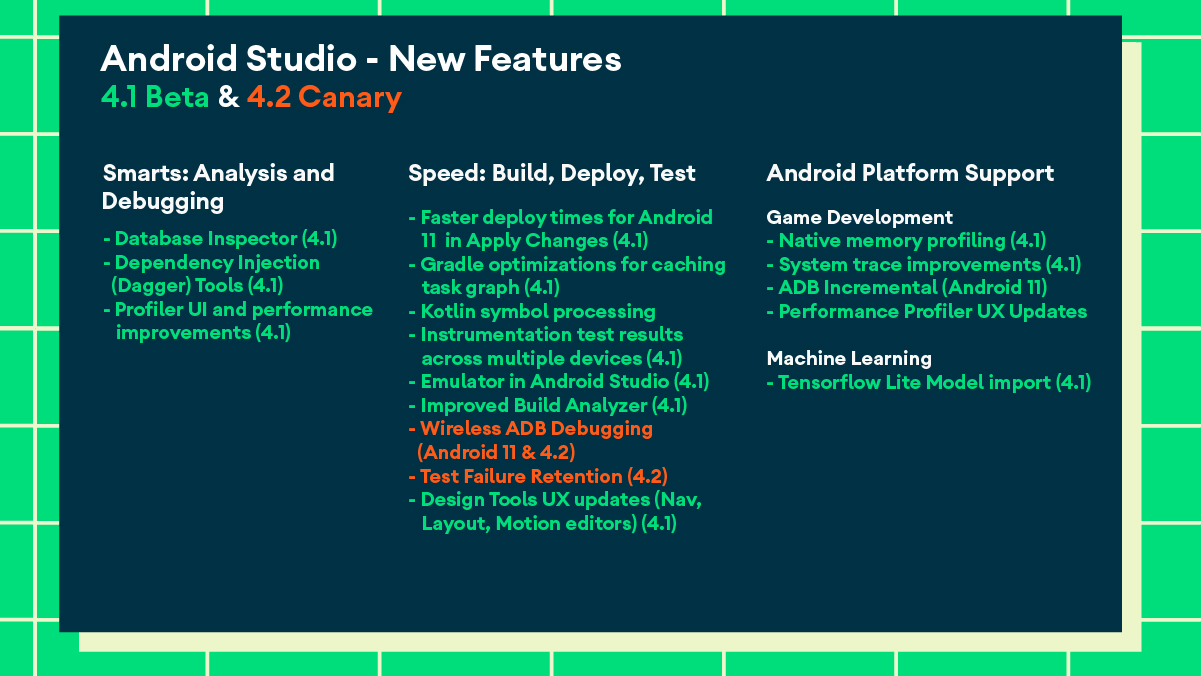
\includegraphics[width=.9\linewidth]{gorseller/android-studio.jpg}
\caption{Android Studio 4.1 Beta ve 4.2 Canary ile gelen özellikler}
\end{figure}

Bu sürümle birlikte gelen diğer özellik ve değişiklikler için konu başlığına
eklediğim ya da yazı içerisinde satır aralarında verdiğim teknik detaylar
bağlantılarına tıklayabilirsiniz. Eğer aramızda Android uygulama geliştirmede
deneyimli arkadaşlar varsa, onlar da yorumlar bölümünde önemli buldukları
özellik ve değişiklikleri vurgulayabilirler.
\section{Visual Studio Code Go eklentisi artık Go projesinin \href{https://blog.golang.org/vscode-go}{parçası haline geldi}}
\label{sec:org0b430ec}
Microsoft tarafından açık kaynak olarak geliştirilen Visual Studio Code metin
editörünün Go programlama dili için olan eklentisi, geçtiğimiz hafta
içerisinde sahibi Microsoft'dan Google'a Go takımına geçti. Eklentinin yeni
depo adresi bu şekilde oldu: \url{https://github.com/golang/vscode-go}. Benim
tahminim artık yeni bir Go sürümü yayınlandığında periyodik olarak aynı
zamanda VS Code Go eklentisi de güncellenecek, böylece de yeni özellikler için
Microsoft'un ilgili takımının ya da açık kaynak topluluğunun geliştirme
yapmasını beklemek gerekmeyecek.

Geçiş ile ilgili Go takımının yazdığı blog yazısına konu başlığına eklediğim
bağlantıya tıklayarak ulaşabilirsiniz.
\section{Apache Software Foundation \href{https://www.youtube.com/watch?v=JUt2nb0mgwg}{belgeseli yayınlandı}}
\label{sec:org573a40f}
\href{https://www.youtube.com/watch?v=JUt2nb0mgwg}{Konuyla ilgili YouTube Videosu}
\section{Visual Studio Code Mayıs 2020 (v1.46) \href{https://code.visualstudio.com/updates/v1\_46}{sürümü yayınlandı}}
\label{sec:org46ecb52}
\begin{center}
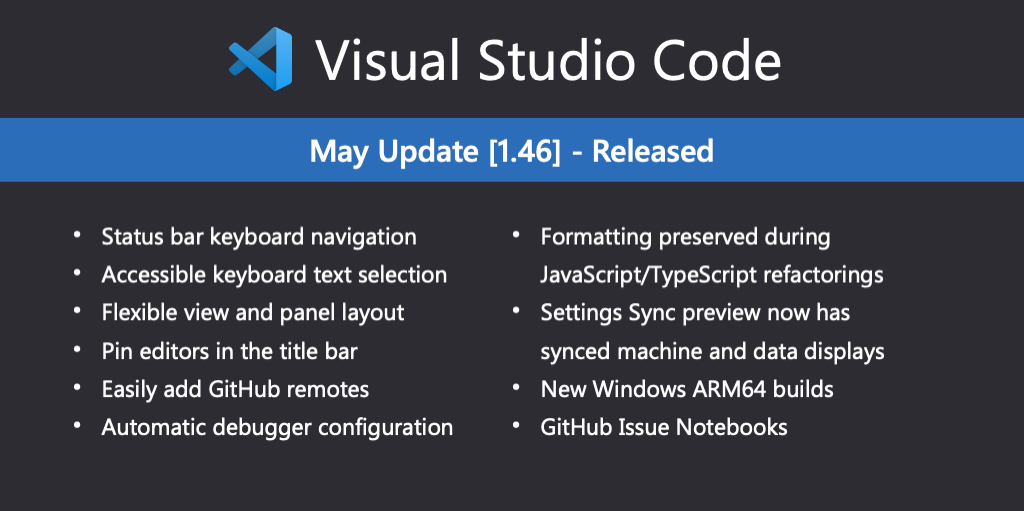
\includegraphics[width=.9\linewidth]{gorseller/vscode-1-46.png}
\end{center}
\section{Yaklaşan Online Etkinlikler}
\label{sec:org20e8626}
\begin{longtable}{|p{9.5cm}|l|}
\hline
Etkinlik İsmi & Tarihi\\
\hline
\endfirsthead
\multicolumn{2}{l}{Önceki sayfadan devam ediyor} \\
\hline

Etkinlik İsmi & Tarihi \\

\hline
\endhead
\hline\multicolumn{2}{r}{Devamı sonraki sayfada} \\
\endfoot
\endlastfoot
\hline
\href{https://kommunity.com/acmhacettepe/events/temel-bulut-bilisim-workshop-ozgur-ozturk-acsdays-1-334aedde}{Özgür Öztürk - Temel Bulut Bilişim Workshop} & 15 Haziran 19:00\\
\href{https://kommunity.com/acmhacettepe/events/powerful-mobile-application-development-veli-bacik-acsdays-2-2f8c2007}{Veli Bacık - Powerful Mobile Application Development} & 15 Haziran 21:00\\
\href{https://kommunity.com/tracikkaynak/events/acik-seminer-35-gun-5g-media-servis-gelistirme-kiti-0589a2f2}{Açık Seminer 35. Gün: 5G-MEDIA Servis Geliştirme Kiti} & 16 Haziran 14:00\\
\href{https://kommunity.com/cozumpark/events/gercek-hayatta-yapay-zeka-1bd98d10}{Gerçek Hayatta Yapay Zeka} & 16 Haziran 14:00\\
\href{https://kommunity.com/acmhacettepe/events/reactjs-ile-web-ve-mobil-uygulamalari-gelistirme-zafer-ayan-acsdays-3-336f845e}{Zafer Ayan - ReactJS ile Web ve Mobil Uygulamaları Geliştirme} & 16 Haziran 19:00\\
\href{https://kommunity.com/bilge-adam-teknoloji/events/spring-boot-rest-service-9f25998f}{Spring Boot REST Service} & 16 Haziran 21:00\\
\href{https://aws.amazon.com/events/summits/online/emea/agenda/}{AWS Summit Online} & 17 Haziran 09:00\\
\href{https://kommunity.com/tracikkaynak/events/acik-seminer-36-gun-5g-use-caseler-ve-5g-3gpp-standarlarindan-nef-8007f5c7}{Açık Seminer 36. Gün: 5G Kullanım Örnekleri ve Kablosuz Haberleşme Ağları} & 17 Haziran 14:00\\
\href{https://kommunity.com/acmhacettepe/events/pandemide-yazilimci-olmak-ender-ahmet-yurt-acsdays-5-af0545e2}{Ender Ahmet Yurt - Pandemide Yazılımcı Olmak} & 17 Haziran 19:00\\
\href{https://kommunity.com/mavidurakio/events/s1e47-yazilimci-bulusmasi-13124b44}{Yazılımcı Buluşması \{MaviDurakIO\}} & 17 Haziran 20:00\\
\href{https://kommunity.com/acmhacettepe/events/sosyal-yonleriyle-acik-kaynak-gelistiriciligi-fatih-kadir-akin-acsdays-6-4ce6fd17}{Fatih Kadir Akın - Sosyal Yönleriyle Açık Kaynak Geliştiriciliği} & 17 Haziran 21:00\\
\href{https://kommunity.com/tracikkaynak/events/acik-seminer-37-gun-3b11c4ed}{Açık Seminer 37. Gün: 5G Nedir?} & 18 Haziran 14:00\\
\href{https://kommunity.com/acmhacettepe/events/performans-neden-onemlidir-bilal-cinarli-acsdays-7-6bdfb155}{Bilal Çınarlı - Performans Neden Önemlidir?} & 18 Haziran 19:00\\
\href{https://kommunity.com/bilge-adam-teknoloji/events/react-native-ile-mobil-uygulama-gelistirme-245c083b}{React Native ile Mobil Uygulama Geliştirme} & 18 Haziran 20:00\\
\href{https://kommunity.com/acmhacettepe/events/yazilim-muhendisliginde-kariyer-harita-arazinin-kendisi-degil-berk-ulsoy-fe3c6d29}{Berk Ulsoy - Yazılım Mühendisliğinde Kariyer} & 18 Haziran 21:00\\
\href{https://kommunity.com/microsoft-student-partners-turkiye/events/lets-meet-with-microsoft-student-partner-ae6f043f}{Let's meet with Microsoft Student Partner Program} & 18 Haziran 21:00\\
\href{https://kommunity.com/tracikkaynak/events/acik-seminer-38-gun-9d1b528b}{Açık Seminer 38. Gün: Haberleşme Teknolojileri Kümelenmesi (HTK)} & 19 Haziran 14:00\\
\href{https://kommunity.com/acmhacettepe/events/sinyal-istihbarati-murat-sisman-acsdays-9-cb66ab0b}{Murat Şişman - Sinyal İstihbaratı} & 19 Haziran 19:00\\
\href{https://kommunity.com/kare-disket/events/web-sitesinin-calisma-prensipleri-ve-temel-html-egitimi-660e1e14}{Web Sitesinin Çalışma Prensipleri ve Temel HTML Eğitimi} & 19 Haziran 20:30\\
\href{https://kommunity.com/acmhacettepe/events/nodejs-deno-ve-js-ile-backend-gelistirmenin-dunu-ve-bugunu-eser-ozvataf-5ef2730a}{Eser Özvataf - Node.js, Deno ve JS ile Backend Geliştirmenin Dünü ve Bugünü} & 19 Haziran 21:00\\
\href{https://kommunity.com/bilge-adam-teknoloji/events/net-core-ile-gercek-zamanli-web-uygulamasi-gelistirme-305ed24d}{.NET Core ile Gerçek Zamanlı Web Uygulaması Geliştirme} & 19 Haziran 21:00\\
\href{https://kommunity.com/devnot-yazilimci-bulusmalari/events/online-microservices-ddd-konferansi-560b28ae}{Online Microservices \& DDD Konferansı} & 20 Haziran 09:30\\
\href{https://kommunity.com/bilge-adam-teknoloji/events/aspnet-web-api-ile-odata-kullanimi-4d505a79}{ASP.NET Web API ile OData Kullanımı} & 20 Haziran 19:00\\
\href{https://kommunity.com/acmhacettepe/events/baran-somakli-freelance-ve-uzaktan-calisma-acsdays-11-004cb0e7}{Baran Somaklı - Freelance ve Uzaktan Çalışma} & 20 Haziran 19:00\\
\href{https://kommunity.com/microsoft-student-partners-turkiye/events/introduction-to-abp-framework-by-ahmet-cotur-fad979a2}{Introduction to ABP Framework by Ahmet Çotur} & 20 Haziran 21:00\\
\href{https://kommunity.com/istanbul-bilisim-toplulugu/events/career-talks-8-oguz-kilic-bir-gelistiricinin-kariyer-yolculugu-93f87bdd}{Career Talks no.8 - Oğuz Kılıç - Bir Geliştiricinin Kariyer Yolculuğu} & 20 Haziran 21:00\\
\hline
\end{longtable}
\section{Diğer Haberler}
\label{sec:orgf1fc003}
\begin{itemize}
\item Cloudflare TV \href{https://blog.cloudflare.com/ladies-and-gentlemen-cloudflare-tv/}{tanıtıldı}. \href{https://cloudflare.tv/live}{Web Sitesi}
\item Apple, WWDC20 \href{https://www.apple.com/newsroom/2020/06/apple-reveals-lineup-for-its-biggest-ever-worldwide-developers-conference/}{etkinliğinin programını açıkladı}.
\item JetBrains Geliştirici Ekosistemi 2020 \href{https://www.jetbrains.com/lp/devecosystem-2020}{anketi sonuçları açıklandı}.
\item Facebook Yapay Zeka takımı, programlama dilleri arasında çevirim yapabilen
\href{https://towardsdatascience.com/facebooks-transcoder-an-ai-source-to-source-compiler-23ea77f3234b}{yapay zeka geliştirdi}. \href{https://arxiv.org/abs/2006.03511}{Akademik Makale}
\item OpenAI takımı yeni yapay zeka \href{https://openai.com/blog/openai-api/}{API araçlarını kullanıma açtı}.
\item AWS yeni \href{https://aws.amazon.com/about-aws/whats-new/2020/06/introducing-aws-codeartifact-a-fully-managed-software-artifact-repository-service/}{hizmetini tanıttı}: \href{https://aws.amazon.com/about-aws/whats-new/2020/06/introducing-aws-codeartifact-a-fully-managed-software-artifact-repository-service/}{AWS CodeArtifact}.
\item GitLab, Peach Teach and Fuzzit \href{https://about.gitlab.com/press/releases/2020-06-11-gitlab-acquires-peach-tech-and-fuzzit-to-expand-devsecops-offering.html}{şirketlerini satın aldı}.
\item DigitalOcean, sorunlar giderilene kadar FRA1 ve NYC3 lokasyonlarında yeni
\href{https://www.digitalocean.com/docs/release-notes/upcoming/spaces-fra1-nyc3/}{Spaces oluşturmayı devre dışı bıraktı}.
\item QUIC ve HTTP/3 destekli özel NGINX sürümü teknoloji \href{https://www.nginx.com/blog/introducing-technology-preview-nginx-support-for-quic-http-3/}{ön izlemesi olarak
tanıtıldı}.
\item .NET 5.0 \href{https://devblogs.microsoft.com/dotnet/announcing-net-5-0-preview-5/}{Preview 5 sürümü duyuruldu}.
\item Valve, OpenXR Geliştirici Ön İzlemesi \href{https://uploadvr.com/valve-openxr-steamvr-beta}{sürümünü yayınladı}.
\item JDK 15 sürümü \href{https://mail.openjdk.java.net/pipermail/jdk-dev/2020-June/004401.html}{Rampdown Phase One aşamasına geçti}.
\item Rust Nightly sürümüne Inline Assembly \href{https://blog.rust-lang.org/inside-rust/2020/06/08/new-inline-asm.html}{desteği geldi}.
\item Dart programlama dili "Null Safety" özelliği \href{https://medium.com/dartlang/announcing-sound-null-safety-defd2216a6f3}{ön izleme olarak duyurdu}.
\item VueJS \href{https://github.com/vuejs/vue-next/releases/tag/v3.0.0-beta.15}{3.0.0 Beta 15 sürümü yayınlandı}.
\item PostgreSQL \href{http://jepsen.io/analyses/postgresql-12.3}{12.3 sürümü yayınlandı}.
\item Apache Flink Stateful Functions \href{https://flink.apache.org/news/2020/06/09/release-statefun-2.1.0.html}{2.1.0 sürümü yayınlandı}.
\item WildFly \href{https://wildfly.org/news/2020/06/08/WildFly20-Final-Released/}{20 sürümü yayınlandı}.
\item Crystal \href{https://crystal-lang.org/2020/06/09/crystal-0.35.0-released.html}{0.35.0 sürümü yayınlandı}.
\item Prisma \href{https://www.prisma.io/blog/announcing-prisma-2-n0v98rzc8br1}{2.0 sürümü duyuruldu}. \href{https://github.com/prisma/prisma}{GitHub Deposu}
\item Linkerd \href{https://linkerd.io/2020/06/09/announcing-linkerd-2.8/}{2.8 sürümü duyuruldu}.
\item Lens \href{https://github.com/lensapp/lens/releases/tag/v3.5.0-rc.1}{3.5.0 RC1 sürümü yayınlandı}.
\item xmake \href{https://github.com/xmake-io/xmake/wiki/xmake-v2.3.4-released,-Better-toolchain-support}{v2.3.4 sürümü yayınlandı}.
\end{itemize}
\section{Lisans}
\label{sec:orgb06b9e6}
\begin{center}
\begin{center}

\includegraphics[height=1.5cm]{../../../img/CC_BY-NC-SA_4.0.png}
\end{center}

\href{yazilim-gundemi-2020-23.pdf}{Yazılım Gündemi - 2020/23} yazısı \href{https://erenhatirnaz.github.io}{Eren Hatırnaz} tarafından \href{http://creativecommons.org/licenses/by-nc-sa/4.0/}{Creative Commons
Atıf-GayriTicari-AynıLisanslaPaylaş 4.0 Uluslararası Lisansı} (CC BY-NC-SA 4.0)
ile lisanslanmıştır.
\end{center}
\end{document}
